% !TeX spellcheck = en_GB

\documentclass[10pt,letterpaper,floatsintext]{article}

\usepackage{ccn}
\usepackage{pslatex}
\usepackage{apacite}

\title{Flow experiences during skill acquisition reflect spontaneous blink rate variation}

% FIXME - data and analysis code in a repository

% insert here the call for the packages your document requires
\usepackage{graphics}
\graphicspath{{./Figures/}}
% \usepackage[latin1]{inputenc}
\usepackage{amsmath}
\usepackage{amsfonts}
\usepackage{amssymb}
\usepackage{url}
\usepackage{xspace}
\usepackage{textcomp}
\usepackage{xcolor}
\usepackage{varwidth}
\usepackage{todonotes}
\usepackage{caption}
\usepackage[normalem]{ulem}
\usepackage{xcolor}
\usepackage{varwidth}

\newcommand{\hl}{\textcolor{red!80}}
\newcommand{\CCS}{\textsf{CogCarSim}\xspace}
\newcommand{\nicewidth}{0.75\textwidth}
\newcommand{\tapprx}{\raisebox{0.4ex}{\texttildelow}}

\author{{\large \bf Benjamin Ultan Cowley (ben.cowley@helsinki.fi)} \\
  Cognitive Science, Department of Digital Humanities, University of Helsinki. POBox 9, 00014, Helsinki, Finland
  \AND {\large \bf Roosa Frantsi (roosa.frantsi@helsinki.fi)} \\
	  Cognitive Science, Department of Digital Humanities, University of Helsinki. POBox 9, 00014, Helsinki, Finland
  \AND {\large \bf Pasi P\"{o}l\"{o}nen (pasi.polonen@helsinki.fi)} \\
	  Cognitive Science, Department of Digital Humanities, University of Helsinki. POBox 9, 00014, Helsinki, Finland
  \AND {\large \bf Ville-Pekka Inkil\"{a} (ville-pekka.inkile@helsinki.fi)} \\
	  Cognitive Science, Department of Digital Humanities, University of Helsinki. POBox 9, 00014, Helsinki, Finland
  \AND {\large \bf Jussi Palom\"{a}ki (jussi.palomaki@helsinki.fi)} \\
	  Cognitive Science, Department of Digital Humanities, University of Helsinki. POBox 9, 00014, Helsinki, Finland
  }

% \author[1,2 *]{Benjamin Ultan Cowley}
% \author[1,5]{Jussi Palom\"{a}ki}
% \author[1,3]{Tuisku Tammi}??
% \author[1,3]{Roosa Frantsi}
% \author[1,4]{Ville-Pekka Inkil\"{a}}
% \author[1]{Noora Lehtonen}??
% \author[1]{Pasi P\"{o}l\"{o}nen}
% \author[1,3,5]{Otto Lappi}??

% \affil[1]{Cognitive Science, Department of Digital Humanities, University of Helsinki, Helsinki, Finland}
% \affil[2]{TRUlab, University of Helsinki, Helsinki, Finland}
% \affil[3]{Helsinki Centre for Digital Humanities (HELDIG)}

\pagestyle{plain}

\begin{document}

\maketitle


\section{Abstract}
{
\bf
Striatal dopamine may be reflected in the spontaneous eye blink rate, which could thus serve as a direct correlate of motivation and cognitive control. One focused state of motivation and cognitive control is \textit{Flow}, a multi-component state of `optimal experience' that arises when skill and task demands match. Here we report a longitudinal experiment on the relationship between task performance, spontaneous blink rate, and self-reported Flow. Participants (N = 9) learned to play a novel steering-game task, designed to elicit Flow by matching skill with demand and providing clear goals and feedback. Our results show that spontaneous blink rate relates to the individual rate of learning, and that this relationship is moderated by Flow, potentially suggesting a role for fluctuations of striatal dopamine in the capacity to perform a learned task at high levels.
}
\begin{quote}
\small
\textbf{Keywords:}
spontaneous blink rate; Bayesian analysis; Flow; skill learning; visuomotor task; high performance cognition
\end{quote}


\section{Introduction}

Spontaneous eye blink rate (sEBR) is a putative index of striatal dopamine \cite{Slagter2012}, and thus may serve as a correlate of motivation and cognitive control. Since these are very broad cognitive domains, it is interesting to examine more constrained states where the 3-way relationship between task, cognition, and neural correlates is more amenable to experimental investigation. For example, Flow is a multi-component state of `optimal experience' \cite{Csikszentmihalyi1975}, the conditions and outcomes of which reflect distinct states of motivation and cognitive control.

One issue with experiments in such domains is that the self-report data required to measure cognitive states is very sparse, by contrast to time-series of physiology or behaviour. Bayesian probabilistic modelling provides a way to examine interaction of performance, physiology, and self-report across complete distributions rather than point estimates, which thus improves capability to infer from sparsely sampled variables.

This paper reports an experimental skill-acquisition study on the connections between performance, physiology, and self-reported Flow, in a novel visuomotor task. Our longitudinal design lets us study how Flow and performance relate to sEBR within- and between-subjects, and we use Bayesian models to examine the interactions in detail. Our Research Questions (RQs) are:

% spontaneous eye blink rate (sEBR) was of interest in our reinforcement-based learning task (positive reinforcement from increase in speed, negative reinforcement from collisions

% Conditions are: {\sf C1} challenges match skill in a demanding task; {\sf C2} clear meaningful goals; and {\sf C3} unambiguous feedback. If Flow arises, self-reported outcomes include: {\sf F1} total focus in the present moment; {\sf F2} merging of action and awareness; {\sf F3} a sense of effortlessness and automaticity; {\sf F4} sense of control; {\sf F5} positive affect; {\sf F6} distortion of temporal experience \cite{Nakamura2002,Engeser2012intro,Keller2012}. %Flow has an autotelic quality, i.e. people want to do Flow-producing activities for their own sake regardless of external reward.
%
% The antecedent conditions ({\sf C1-3}) and phenomenological features ({\sf F1-6}) of Flow have been investigated for several decades, mainly using analysis of self-report data from participants engaging in natural everyday or expert performance \cite{Csikszentmihalyi1971,Moneta2012}...
%
% Prior Flow research has tended to capture a static snapshot of Flow, so we must still deal with \textit{learning} that increases skill, and knock-on impact on skill-challenge balance.
%
% %anticipate MAIN RESULT and its IMPLICATIONS here
% ... understanding the specific mechanisms that mediate Flow and learning could be significant for enhancing enjoyment or performance in many tasks.
%
% ... call for studies of Flow as elicited in different phases of learning, with a more controlled and quantitative approach; i.e. using approaches from experimental psychology \cite{Harris2017,Keller2008}, and psychophysiology \cite{Peifer2012,Peifer2014,Wolf2015,Harmat2015,Labonte-LeMoyne2016}.

\begin{enumerate}
	\item RQ1. Does the median baseline sEBR of each participant relate to their performance and Flow experience?

	\item RQ2. Does sEBR variation across sessions (of each participant) affect their perceived cognitive performance, i.e. Flow, perceived importance, skill:demand?

\end{enumerate}

Unrelated RQs regarding behavioural data have been published elsewhere \cite{Cowley2019flow}; that article also gives a more in-depth description of the experiment.

%%%%%%%%%%%%%%%%%%%%%%%%%%%%%%%%%%%%%%%%%%%%%%%%%%%%%%%%%%%%%%%%%%%%%%%%%%%%%%%%
%%%%%%%%%%%%%%%%%%%%%%%%%%%%%%%%%%%%%%%%%%%%%%%%%%%%%%%%%%%%%%%%%%%%%%%%%%%%%%%%
%%%%%%%%%%%%%%%%%%%%%%%%%%    METHODS    %%%%%%%%%%%%%%%%%%%%%%%%%%%%%%%%%%%%%%%
\section{Methods}

\paragraph{Overview:}
Participants learned to play a custom-made high-speed steering game (for game video see \url{https://doi.org/10.6084/m9.figshare.7269395.v1}). The aim of the game was to steer a blue cube through a course with randomly placed red obstacles at the highest possible speed, so performance was measured by duration of the trial. Collision with obstacles reduced speed by a fixed amount. The cube started each game at a fixed forward velocity, which increased at a constant rate. The lateral position of the cube was controlled by steering wheel. The game was specifically designed to elicit Flow by constantly balancing task demand with participant skill, and providing clear immediate feedback.

Participants played the game for forty trials across eight sessions, over a period of 2-3 weeks, giving total play time = $~$2h which was sufficient to achieve good proficiency in this task with no ceiling effect. The 10 item Flow Short Scale \cite{Engeser2008} was filled after each trial. Physiological data were recorded, during task and five minutes of baseline, in sessions one and five-to-eight.


\paragraph{Participants}
A convenience sample (N=9, 6 males, 3 females) was recruited, between 22-38 years of age (mean 27, SD 3), with normal or corrected-to-normal visual acuity and no history of neurological or psychiatric disease. All participants were naive about the specific hypotheses and purpose of the study; they were remunerated for their time. Participants were briefed and gave written informed consent before the study. The study followed guidelines of the Declaration of Helsinki and was approved by the University of Helsinki Ethical review board in humanities and social and behavioural sciences (statement 31/2017; study title MulSimCoLab).

\subsection*{Materials}
\paragraph{Task \& Equipment} Participants played the custom high-speed steering game {\it CogCarSim} (game code permanently available under open source licence at \url{https://doi.org/10.6084/m9.figshare.7269467}). Separate computers were used to run the game and record the physiology data.

Participants were seated aligned with the mid point of a 55" display screen (LG 55UF85), resolution 1920$\times$1080 pixels, refresh rate 60Hz. Eye-to-screen distance was 90--120 cm.

For physiological measurement sessions (1,5,6,7,8), participants were dressed in sensors, seated in the driving seat in quiet, low-light conditions for baseline measurement, where they sat still for five minutes looking at a dark blue screen.

We used Pupil Labs Binocular 120 Hz eye tracker (Pupil Labs UG haftungsbeschr\"{a}nkt, Berlin, Germany), stabilised with a custom-built headband, with data acquisition via Pupil Capture software. Gaze direction was calibrated using ten markers on the display, three times per session.

Electrodermal activity (EDA, not reported here),  was recorded from the left foot (to minimise motor artefacts). Blood volume pulse (BVP) was measured using a pulse oximeter sensor attached to the left index toe.

\paragraph{Flow Short Scale} To measure self-reported Flow, participants filled the Flow Short Scale (FSS) after each trial \cite{Cowley2019flow}. The response format of FSS is a 7-point Likert scale ranging from lower to higher values of the item (e.g. higher scores indicate higher experienced Flow/PI). FSS has 10 core items which load subfactors {\it fluency of performance} (6 items) and {\it absorption by activity} (4 items); these subfactors were averaged to obtain Flow scores. There were also 3 items (here analysed separately) for {\it perceived importance} (PI) -- 1. \textit{Something important to me is at stake here}; 2. \textit{I must not make any mistakes here}; 3. \textit{I am worried about failing}.

% (+3 additional items)
In addition to these 13 items asked after every trial, after each session participants were asked 3 items measuring skill and demand. The demand item (\textit{Compared to all other activities which I partake in, this one is...(easy - difficult)}) was subtracted from the skill item (\textit{I think that my competence in this area is...(low - high)}) to code a skill-demand variable.
% These items, plus the 3 PI items, were used separately in analyses.


\subsection*{Analysis}
Data for RQ1 were aggregated at participant level. Learning curve (LC) was derived by fitting power-law models to the trial-duration scores distributed over runs, then log-transforming to obtain linear models. Analyses reported here use LC slopes.

RQ2 is addressed by session-wise data, with parameters gathered either directly at the session level (sEBR, skill:demand self-reports), or aggregated from run-level data (Flow and PI self-reports).
%FIXME: REPORT WHICH VARS WERE CENTERED OR SCALED?
%FIXME: EXPLAIN WHAT FINAL VARIABLES WERE USED!

\paragraph{Signal preprocessing}
Eye blinks were counted manually from the middle three minutes of each baseline eye-tracking video (from sessions 1 \& 5--8). Four of 40 baselines were excluded due to measurement problems.

All fast and simultaneous movements of both eyelids were counted as blinks (even if the eyelid did not fully close). To ensure rater reliability, two authors independently counted the number of blinks in sessions 1, 6 and 8. Inter-rater reliability of their counts was calculated as 98.7\% (see below); thus, blinks in sessions 5 and 7 were counted by only one experimenter.

We calculated the level of consensus between the two raters as follows. Separately for each participant and session, we divided the difference of two raters' blink counts by the mean of those counts, and then subtracted the quotient from 1 to obtain a percentage. These were averaged to give total inter-rater reliability. The session-wise reliability scores also had low variability (mean of standard deviations = 0.01). The final sEBR was calculated as median blinks per minute during the three minutes counted.

\paragraph{Statistical methods:}
All analysis was implemented with {\bf R} platform for statistical computing. {\it p}-values were corrected for multiple comparisons using Bonferroni-Holm. {\bf R} code and data used to produce all analyses and figures is permanently available online at 
\todo{FIXME - NEW .Rmd FOR BLINK PAPER}

Each RQ was addressed both by linear regression for comparison, and by Bayesian modelling to explore the space of models, select the best fit, and examine the interactions. 

\paragraph{Linear analyses:}
For {\bf RQ1} we modelled main effects and interaction of Flow and LC as predictors of sEBR by linear regression. We then conducted simple slopes interaction (SSI) analysis (with {\bf R}'s {\bf jtools} package), estimating slope of LC when Flow was held constant at its mean$\pm$1SD. 

For \textbf{RQ2} we used (restricted maxmimum likelihood) Linear Mixed Models (LMMs) with random effect of participant (using {\bf lmer} package for {\bf R}). SSI analysis estimated the slope of PI-2 when skill-demand was held constant at its mean$\pm$1SD.

\paragraph{Bayesian analysis:}
Bayesian inference methods were used to sample from the joint posterior distribution of model parameters for performance, sEBR, and self-report data, as per $p(\theta|D) \propto p(D|\theta)p(\theta)$. We thus constructed models for each combination of relevant parameters, starting with the intercept-only model and ending with two-way interactions.  

% \begin{equation}
%     p(\theta|D) \propto p(D|\theta)p(\theta)
% \end{equation}

All models were fit with Stan probabilistic programming language, utilising No-U-Turn Hamiltonian Monte Carlo sampler. {\bf brms}-package was used for model fitting. All model priors were defined as generic weakly informative. We used Leave-One-Out (LOO) cross-validation method for model comparisons and selection by predictive accuracy.

\todo[author=VPI]{TODO: CHECK BAYESIAN METHODS}

%%%%%%%%%%%%%%%%%%%%%%%%%%%%%%%%%%%%%%%%%%%%%%%%%%%%%%%%%%%%%%%%%%%%%%%%%%%%%%%%
%%%%%%%%%%%%%%%%%%%%%%%%%%%%%%%%%%%%%%%%%%%%%%%%%%%%%%%%%%%%%%%%%%%%%%%%%%%%%%%%
%%%%%%%%%%%%%%%%%%%%%%%%%%    RESULTS    %%%%%%%%%%%%%%%%%%%%%%%%%%%%%%%%%%%%%%%
\section{Results}
% Multiplicity correction
% nhst#         tests   pvals    padj
% 1           sEBRxLC 0.21480 1.00000
% 2         sEBRxFlow 0.70000 1.00000
% 3    FlowXresiduals 0.00300 0.04500
% 4  sEBRxLCxFlow+1SD 0.00001 0.00018
% 5 sEBRxLCxFlow_mean 0.00001 0.00018
% 6  sEBRxLCxFlow-1SD 0.15000 1.00000
% 7  sEBRxLCxFlow LMM 0.00074 
% 8 sEBRxPI2xSkDm+1SD 0.00001
% 9  sEBRxPI2xSkDm_mn 0.33000
% 10 sEBRxPI2xSkD-1SD 0.12000

\todo{Recalculate adjusted p-values}

\paragraph{RQ1: Is sEBR related to performance or Flow?}

sEBR showed a negative relationship to participant-wise LC slopes, as shown in Fig.~\ref{fig:EBRvLC}, panel A. The correlation is of moderate strength, though non-significant (Pearson's {\it r} = -.46 , {\it p} = 1.0, N = 9). %NHST1
The LC slope of every participant was negative, which means we can say that the smaller the sEBR, the shallower the LC slope.% Or, because slope and intercept are highly correlated, it is almost equivalent to say that smaller sEBR correlates with better initial performance.


Mean Flow scores are not directly related to sEBR (Pearson's {\it r} = 0.15, {\it p} = 1.0, N = 9). %NHST2
%%%% FLOW X SEBR COR TEST
% data:  FM and sEBR
% t = 0.41014, df = 7, p-value = 0.694
% alternative hypothesis: true correlation is not equal to 0
% 95 percent confidence interval:
%  -0.5688016  0.7418380
% sample estimates:
%      cor
% 0.153187
However, examining Fig.~\ref{fig:EBRvLC} shows an interesting relationship: the residuals of the fitted linear model (i.e. vertical distance of each data-point from the line) are {\it strongly} related to mean Flow scores (Pearson's {\it r} = -.86 , {\it p} = .04, N = 9). %NHST3
%%%% FLOW X RESIDUAL COR TEST
% data:  FM and abs(LC - LM$fitted.values)
% t = -4.4556, df = 7, p-value = 0.002952
% alternative hypothesis: true correlation is not equal to 0
% 95 percent confidence interval:
%  -0.9700331 -0.4562393
% sample estimates:
%       cor
In other words, participants' mean Flow scores are strongly correlated with their observed deviation from the linear relationship between sEBR and task learning (LC slope). This correlation is not driven only by the non-significant correlation of Flow and LC (above). In fact, interaction analysis (see Table~\ref{tab:simpslopes}) shows that when Flow mean is above 5.05, LC slope significantly predicts sEBR at {\it p} $<$ 0.0001. %NHST4+5
% SIMPLE SLOPES ANALYSIS
% Slope of LC when FM = 5.40 (+ 1 SD):
%      Est.   S.E. t val.    p
%  -1096.31 221.36  -4.95 0.00
% Slope of LC when FM = 5.06 (Mean):
%     Est.   S.E. t val.    p
%  -683.33 143.15  -4.77 0.00
% Slope of LC when FM = 4.73 (- 1 SD):
%     Est.   S.E. t val.    p
%  -270.35 158.23  -1.71 0.15

In the \textbf{Bayesian} approach, according to the LOO model comparisons, the LC$\times$Flow interaction model had the best out-of-sample predictive accuracy. Visual diagnostics (created using \verb|brms::pp_check| function; not shown due to space constraints) indicated acceptable fit for the posterior predictive distribution. Model diagnostics (Eff.Sample = 1825 and Rhat = 1.0) indicate acceptable level of convergence. For this model, the 95\% Highest-Density Interval (HDI) of the posterior sample distribution is -0.86..-0.15, so the interaction effect is non-zero. Fig~\ref{fig:EBRvLC}, panel C, shows the modelled interaction (created using \verb|brms::marginal_effects|).


\begin{figure*}[!t]
	\centering
	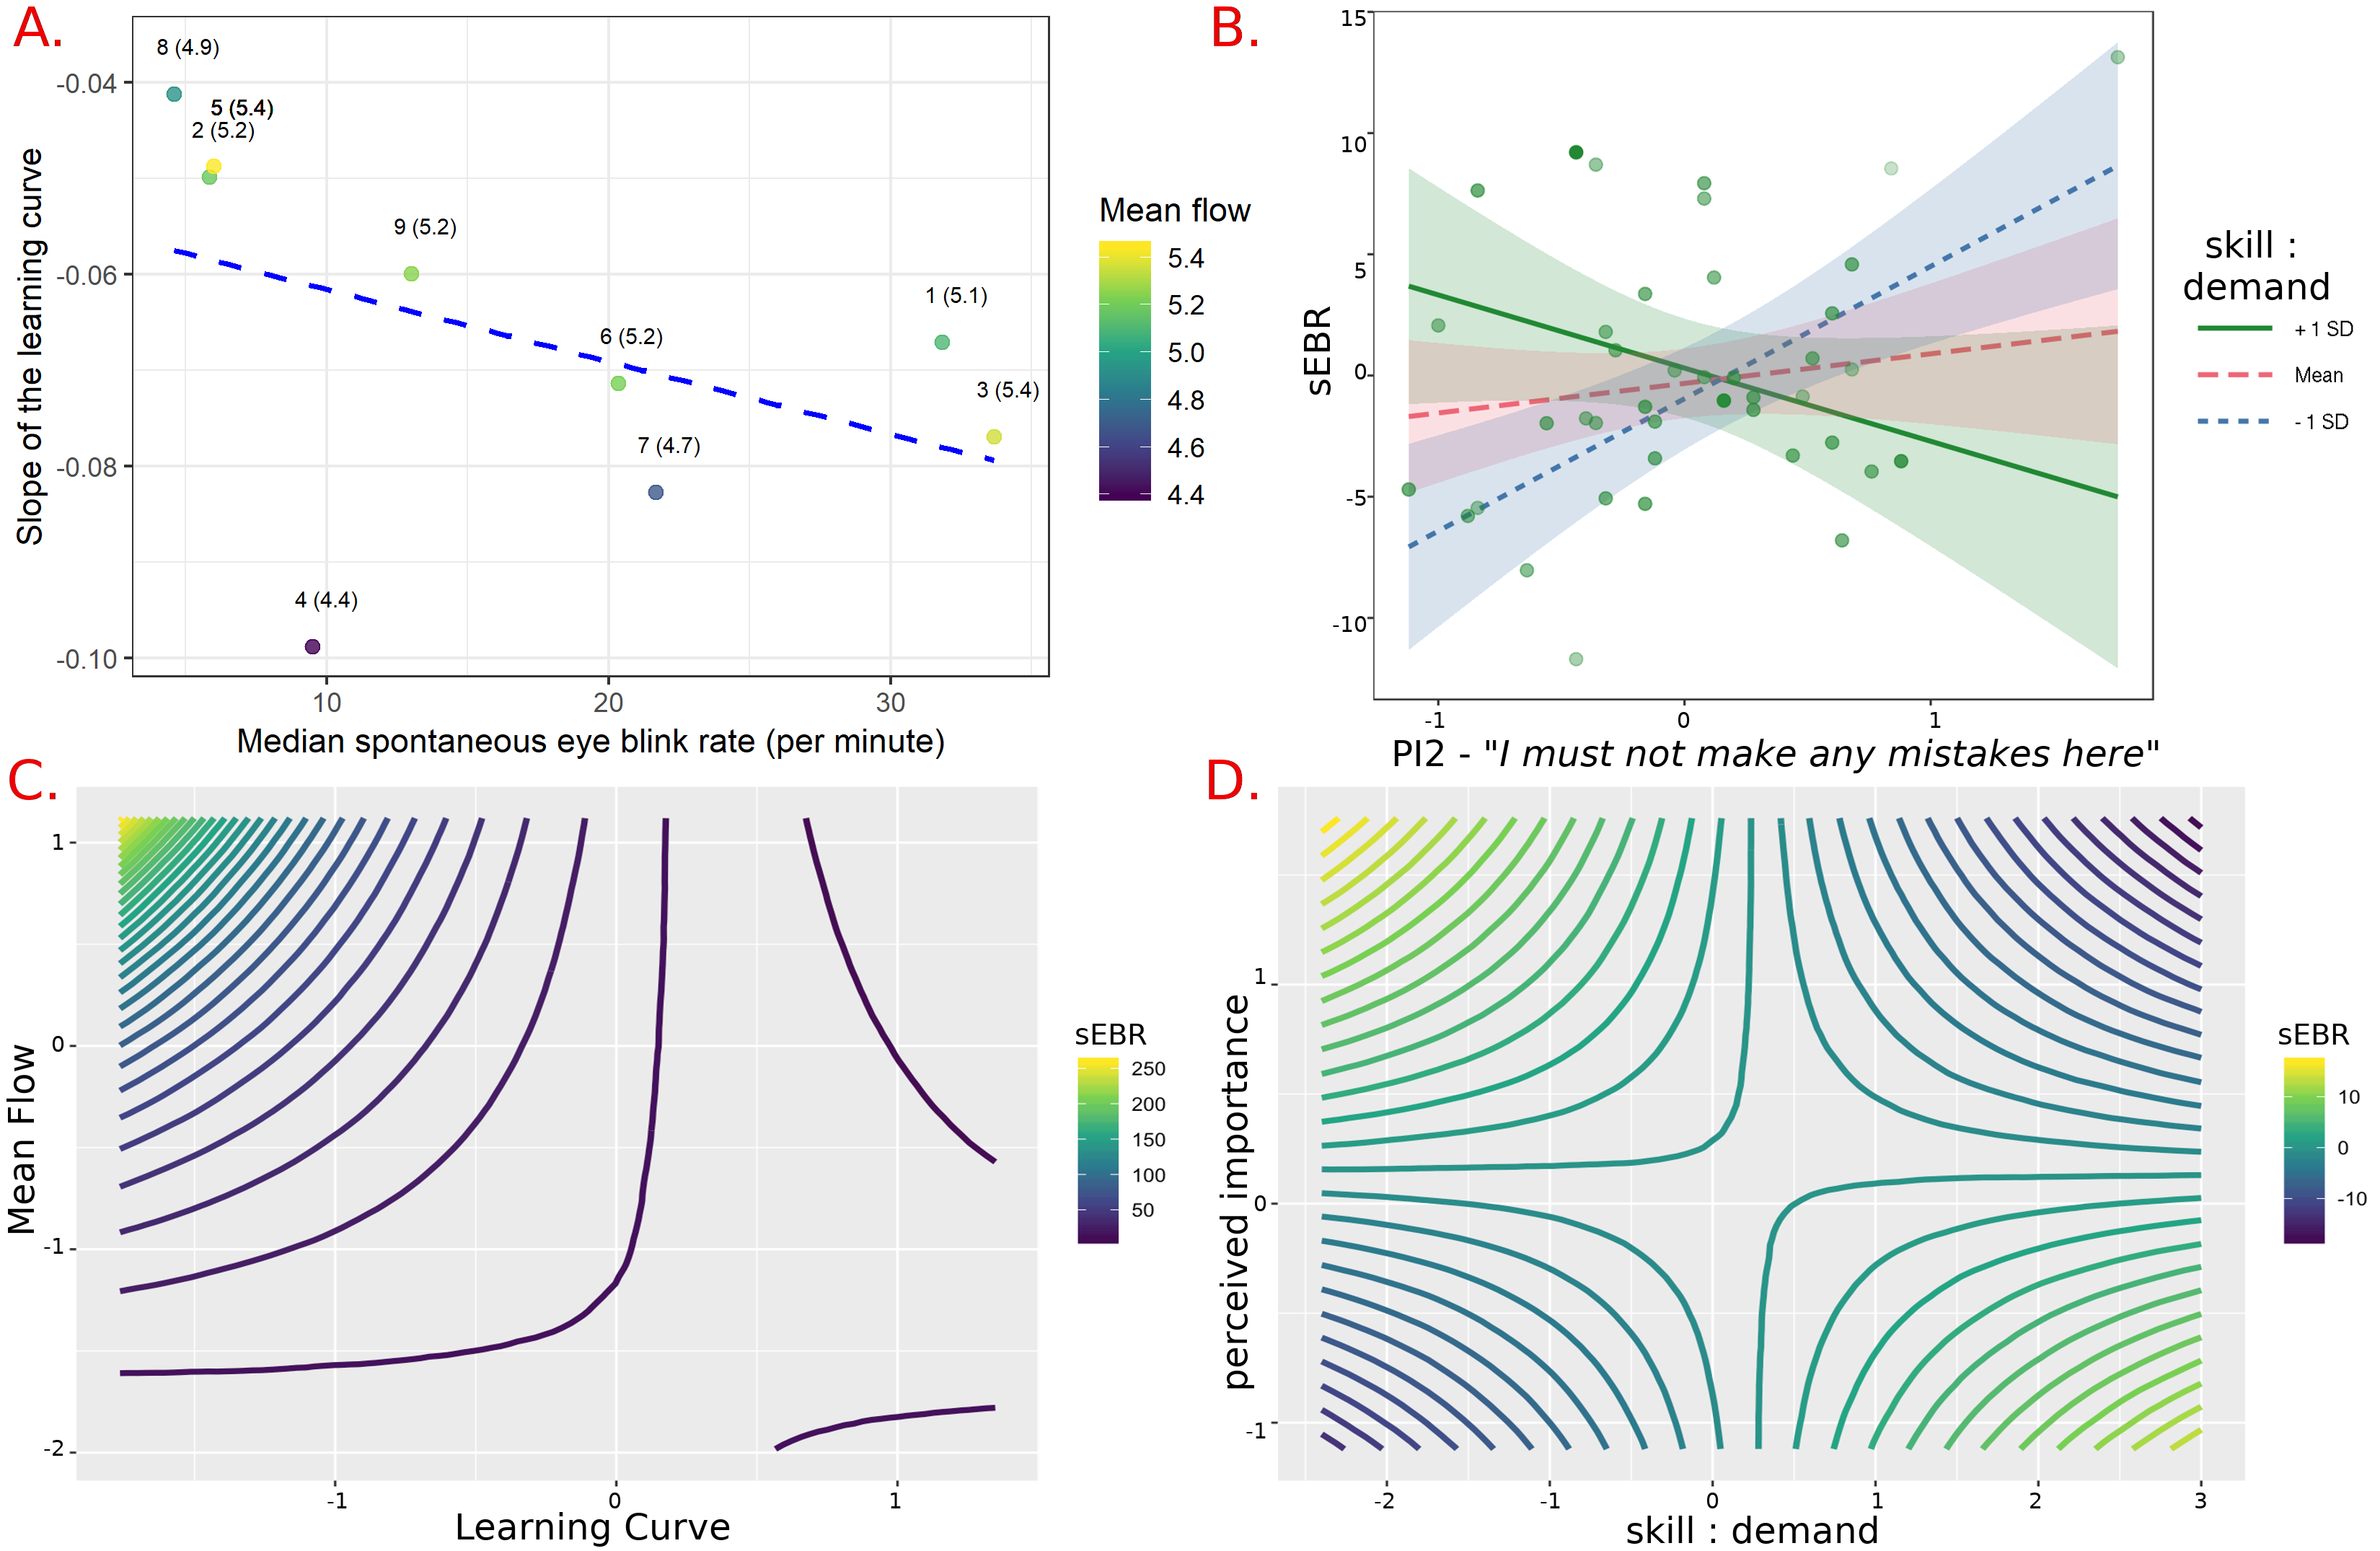
\includegraphics[width=\textwidth]{sEBR_RQ1-2_results}
	\caption{\textbf{Panel A}: Participants' median spontaneous eye blink rate plotted against the slope of their learning curve, and coloured by their mean Flow scores. Linear model is depicted by the dashed line. Each point is labelled with the participant number (1..9) and exact mean Flow score (in parentheses). \textbf{Panel B}: ... \textbf{Panel C}: ... \textbf{Panel D:} ...}
	\label{fig:EBRvLC}
\end{figure*}


\begin{table}[!hb]
\centering
\caption{Outcome of simple-slopes analysis for participant-wise Flow$\times$LC interaction: each row reports on the slope of LC slope at the level and value of Flow shown.}
\begin{tabular}{llllll}
\hline
Flow level & Flow & Est. & S.E. & t value & p \\
\hline
+ 1 SD & 5.40 & -1096.31 & 221.36 & -4.95 & 0.0002 \\
Mean   & 5.06 &  -683.33 & 143.15 & -4.77 & 0.0002 \\
- 1 SD & 4.73 &  -270.35 & 158.23 & -1.71 & 1.0 \\
\hline
\label{tab:simpslopes}
\end{tabular}
\end{table}

\paragraph{RQ2: session-wise sEBR and self-report}
LOO testing of Bayesian models showed best out-of-sample predictive accuracy for interaction model with parameters skill-demand and PI-2 (``\textit{I must not make any mistakes here}''). 
Visual diagnostics (created as above) indicated acceptable fit for the posterior predictive distribution. Model diagnostics (Eff.Sample = 4369 and Rhat = 1.0) indicate acceptable level of convergence. For this model, the 95\% HDI of the posterior sample distribution is -6.41..-1.83, so the interaction effect is non-zero. Fig~\ref{fig:EBRvLC}, panel D, shows the modelled interaction (made by \verb|brms::marginal_effects|).

The skill-demand$\times$PI-2 LMM predicting sEBR showed the interaction was significant (df = 37, t = -3.680, p < 0.001). %NHST7
Fig.~\ref{fig:EBRvLC} panel D shows the interaction at fixed levels of skill-demand (created by \verb|jtools::interact_plot|). SSI analysis shows that when (self-rated) demand exceeds skill the PI-2 slope significantly predicts sEBR at {\it p} $<$ 0.0001. %NHST10


%%%%%%%%%%%%%%%%%%%%%%%%%%%%%%%%%%%%%%%%%%%%%%%%%%%%%%%%%%%%%%%%%%%%%%%%%%%%%%%%
%%%%%%%%%%%%%%%%%%%%%%%%%%%%%%%%%%%%%%%%%%%%%%%%%%%%%%%%%%%%%%%%%%%%%%%%%%%%%%%%
%%%%%%%%%%%%%%%%%%%%%%%%     DISCUSSION    %%%%%%%%%%%%%%%%%%%%%%%%%%%%%%%%%%%%%
\section{Discussion}
% exploration of Flow and on-task learning (LC as opposed to pre- post)
Based on a longitudinal experiment of Flow in a game-like high-speed steering task, we report evidence that LC slope is predicted by the participants' spontaneous blink rate, moderated by global Flow. This relationship potentially indicates a role for striatal dopamine in learning the visuomotor steering task, which may interact with experiential aspects. We further examined interactions between learning, sEBR, and perceived skill:demand balance and importance....%FIXME: REPORT RQ2


% Relation to previous Work on eye blink rate
\paragraph{RQ1 - Learning, Flow, and sEBR:}
Evidence for RQ1 suggests a clear linear trend relating sEBR and LCs (Fig.~\ref{fig:EBRvLC}): the larger the sEBR, the steeper the LC slope (or: the higher the LC intercept). The distance of data-points from the fitted model values also closely match the distribution of Flow mean scores, meaning that individuals with lowest Flow also diverge the most from the sEBR$\times$LC model. Interaction analysis then supports the idea that sEBR correlation with LC is stronger the higher the mean Flow. We thus claim that there is a genuine sEBR--LC relationship that is moderated by Flow. We cannot decide causality based on our data, but there is literature relevant to mechanisms, that can help identify future directions of inquiry.

Learning is influenced both by psychological factors (motivation, prior experience) and physio-/neurological factors. One potentially relevant factor for studying Flow and skill acquisition is the well-established relationship between attention and striatal dopamine levels \cite{Dreisbach2005}. The striatum plays a major role in decision making and reward/aversion processing, moderated by the level of tonic dopamine D2-receptors therein; the postsynaptic levels of dopamine can thus bias the entire learning process. This is illustrated for example in studies of `attentional blink' (AB) by Slagter and others \cite{Slagter2012,COLZATO2008}), which suggest a U-shaped function between tonic striatal dopamine and AB size. In other words, very high or low levels of dopamine D2-receptor density can make attention updating too rapid (distractable) or too slow (inattentive).

sEBR has been suggested as an externally-measurable index of striatal dopamine level (though caution is needed, see \cite{dang2017spontaneous}). Early work by \cite{Karson1983} linked sEBR to striatal dopamine in humans and other primates. \cite{Taylor1999} then localised to the caudate nucleus, whose normal function is implicated in classification learning \cite{Seger2005}; caudate nucleus volumetric asymmetry is implicated in inattention symptomatology \cite{Schrimsher2002}. Later work from \cite{Slagter2015} has shown that sEBRs may relate specifically to avoidance learning; others have linked dopamine levels and sEBR to perseverance, distractibility and cognitive control \cite{Muller2007,Dreisbach2005}. Finally, \cite{DeManzano2013} have shown that  predisposition to experience Flow is positively correlated with striatal dopamine D2-receptor availability (measured in PET), specifically in caudate and putamen, and stronger in right hemisphere than left.

Let us consider learning as a process whereby perception, cognition and action become attuned to task demands. In our game task, learning involves high-frequency decision making with respect to continuously updating stimuli of uniform kind (not unlike AB task, a continuous performance test designed to probe AB size \cite{Slagter2012}). In this view, the sEBR--LC relationship could be interpreted as showing that higher D2 density indexed by sEBR supports learning (LC slope). An alternative interpretation is that it reflects higher distractability in the early phases of learning (LC intercept).

The underlying mechanism could be that higher dopamine levels permit more rapid attention updating and thus more fluid response to changing task demands. This can work despite \cite{Slagter2012}'s proposed U-shaped function: because our game-task constantly maintains a level of demand slightly greater than the participants' skill. Thus, in this context, higher sEBR tends to be better, possibly because the {\it requirement} for rapid attention updating grows with the learned task skill.

Less subjective Flow was reported by those participants who deviated (positively or negatively) from this relationship. Lower Flow could be due to, e.g., misalignment of task demands and attentional updating rate, creating a more effortful experience. So the observed moderation by Flow scores of the sEBR--LC relationship could be speculated to have a basis in adjusting attention updating, in response to changing task speeds, physiologically underpinned by the nigro-striatal DA system. In other words, it may not be the case that an absolute level of striatal dopamine should predict learning, but rather an individual level relative to how each participant relates to the task (vis-\'{a}-vis gaming experience, motivation, fine motor skills, or potentially many other variables). If a participant's tonic dopamine is not at their ideal level for this task, they might nevertheless do well in the task, and yet find the experience more effortful and less fluid (than is suggested as Flow-like by wording of the FSS).


% \subsection{Limitations and Future Work}
To further explore the possible role of striatal dopamine, it would be interesting to experimentally manipulate the game to adjust the distance between obstacles, thus altering the attention-updating rate required to navigate without collisions (motor precision variation can be minimised by a suitably long training period). This manipulation could be varied in response to measurements of sEBR (which can be automated, e.g. by using electro-oculography \cite{toivanen2014}), to systematically study if sEBR has explanatory power for individual variability in learning.



%%%%%%%%%%%%%%%%%%%%%%%%%%%%%%%%%%%%%%%%%%%%%%%%%%%%%%%%%%%%%%%%%%%%%%%%%%%%%%%
%%%%%%%%%%%%%%%%%%%%%%%%%%%%%%%%%%%%%%%%%%%%%%%%%%%%%%%%%%%%%%%%%%%%%%%%%%%%%%%%
%%%%%%%%%%%%%%%%%%%%% POST-HOC MATERIAL OF VITAL IMPORTANCE %%%%%%%%%%%%%%%%%%%%


\section{Acknowledgements}
We thank Tuisku Tammi, Noora Lehtonen, Otto Lappi, Kalle Toika, and Juha Veps\"{a}l\"{a}inen.

% \section*{Author contributions statement}
% % please edit as appropriate
% OL, JP and BUC conceived the study.
% OL helped design the gameplay.
% BUC and TT designed and implemented the data collection.
% NL, TT, PP, RF, VPI, and JP translated the FSS.
% All authors participated in decisions on the experiment specifications.
% RF, VPI, NL, PP, and TT conducted the experiment.
% BUC, VPI, TT, RF, PP, NL, JP, and OL analysed and interpreted the results.
% BUC, JP and OL drafted the paper.
% All authors participated in writing and reviewing, and approved the manuscript.


\bibliographystyle{apacite}

\setlength{\bibleftmargin}{.125in}
\setlength{\bibindent}{-\bibleftmargin}

\bibliography{CogCarFlow_bib}

\end{document}
